%!TEX root = main.tex

Greetings, hello, hi, [In voyager, we sent greetings in 55 different languages, which could be cool to merge in one mega greeting/goodbye]

We are individuals from a star system far from yours. 
%, the location of which would be too complicated to describe given your current understanding of the universe. 
We have been assigned by our society the role of surveying the diversity of life forms across our galaxy and have been systematically visiting planets that appear suitable to sustaining life similar to ours. We identified this star system as a possible life-supporting system. As such, we decided to voyage close to this location to assess its viability.
%, planet to planet, for around 30 earth years. Do not worry, we live up to 160 earth years. 
During our latest hyperdrive jump, we nearly collided with a small vessel made by a lifeform unknown to us. Deconstructing this object, we discovered within it a flat golden disk, and upon following the instructions printed on the disk, decoded the information etched into it by your society. 

By studying the stellar diagram on the disk, and cross-referencing this with the ratio of uranium-238 atoms found in the vessel, we realized that your home star system was extremely close to our present location but had been undetected by us because it bears so little in common with our own star system. This fortuitous discovery has allowed us the opportunity to study what kinds of lifeforms can evolve in this seemingly hostile environment. 

The golden disk already contained a great deal of information about you. You appear to understand a subset of mathematical logic and the processes that govern the physical world, which is impressive. There is great diversity in the traits of your life forms, though we did not understand much of what the images depicted. The auditory signals on the disk were intriguing -- some of these signals appear quite sophisticated, such as that labeled ``whale'' and ''Chuck Berry,'' while others are primitive, such as ``Mozart.'' Incidentally, there is, in fact, a 'Turkish'-speaking individual among our crew, who responds to your message with: [Gizem insert something here?]. 

Of all of the information encoded in your disk, however, one feature surprised us most: your apparent reproductive system. Among the images, we found one which depicts two individuals, who look somewhat different from each other and are labeled with symbols (Figure~\ref{fig:1}). The same symbols appeared next to other life forms that different greatly in size and shape (Figure~\ref{fig:2}). These and other images suggest three facts: i) there exist two mating types, ii) one of each mating type is required for reproduction, and iii) the mating types have very different properties. We have, in fact, never observed this in any of the other life forms that we have encountered. Until now we believed that three or more individuals were required for reproduction.

This highly unusual feature of your biology convinced us to study the conditions that may have produced a biparental reproductive system and the consequences of such a system, compared to the more familiar triparental system. We studied your methods of measurement, logic, and communication to gain the ability to transmit our own message to you. Here, we use your units of measurement, your notational system for recording mathematical ideas, and your format for recording knowledge so that you may understand us. Unfortunately, our trajectory only permits a detour of 72 hours, so we are only able to give brief descriptions of our most important findings. 

As we approached your star system, we observed that you use electromagnetic radiation to communicate. We reverse-engineered this communication modality to access your store of knowledge and to relay our own message to you. In this document, we reference knowledge from your own culture that will help you to understand the knowledge that we present to you. We wanted to deposit our message at a location that will ensure that you detect it. One image on your golden disk depicts a structure that appears designed to receive and amplify weak electromagnetic signals (the ``Taj Mahal''). A survey of the surface of your planet revealed an even more optimal signal receiving structure, located near the village of Santa Fe, New Mexico, USA (Figure~\ref{fig:3}). An optical scan of this structure showed it to be inhabited by fourteen of your life forms, and our message has therefore been sent to this location with the hope that these individuals will convey our message to rest of your planet. 

%travels [maybe give exact location of voyager I or II?], we came across a slow moving object. Imagine our surprise when we inspected this object, realizing it was intended as a gift for another form of intelligent life. Included in this object was a flat cylindrical disk encoded with sounds (we were fascinated by these sounds you sent: the sound of the whale is beautiful, the sounds of ``Mozart'' were confusing) as well as several images. 

%Within the cylinder we noticed a few dwellings, one located in the area known as New Mexico, and one called the "Taj Majal" which included several domes. Thus we identified a house in New Mexico with dome-structures like this Taj Majal where we are sending our information. While we imagine there are many topics we could discuss, finding commonalities and differences among our InterPlanetary cultures, one struck us in particular. 

%//[maybe more stuff on the golden record and what we liked about it?]

%The drawings you included in your gold colored disk fascinated and intrigued us. The main picture we determine is a type of 'address', showing us your location, as well as who you, as a species, are. There are several sub-pictures included as well. The picture of one large entity (what you call an "egg"), and multiple small entities from another group (what you call "sperm") may suggest that sexual reproduction among your society is between two individuals (Figure~\ref{fig:1}). The next picture seems to imply that the two entities are associated with two different sexes of humans and these two lead to gestating offspring (Figure~\ref{fig:2}). This image implies that only two individuals are required to reproduce, while the next pictures confirms that reproduction requires only two (different types of) humans. This is surprising: we have never seen a world where only two individuals reproduce. 


\begin{figure}
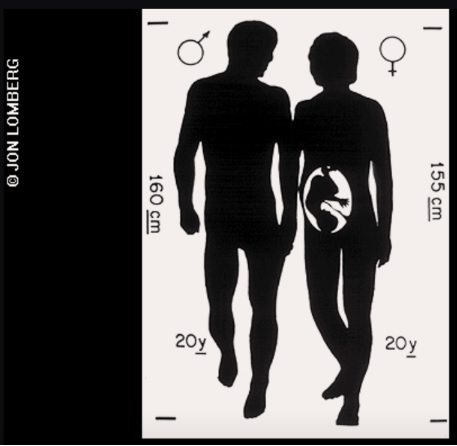
\includegraphics[width=1\columnwidth]{parents_voyager.jpg}
\caption{Two visually distinct life forms, each apparently required for reproduction. Image decoded from the golden disk.
\label{fig:1}}
\end{figure}

\begin{figure}
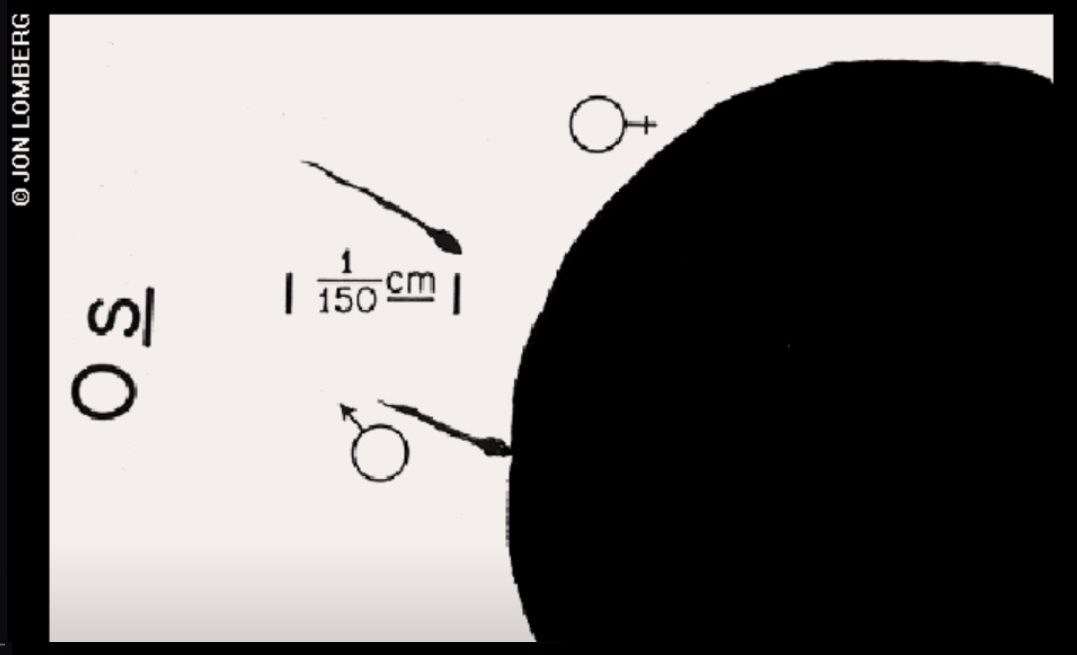
\includegraphics[width=1\columnwidth]{spermandegg_voyager.jpg}
\caption{Entities that are subsets of the life forms depicted in Figure~\ref{fig:1}. These apparently function as the direct mechanisms leading to reproduction and exhibit extremely large size differences. Image decoded from the golden disk.
\label{fig:2}}
\end{figure}

\begin{figure}

\includegraphics[width=1\columnwidth]{rassMandal.jpg}
\caption{Optimal electromagnetic signal receiving structure in Santa Fe, NM.
\label{fig:3}}
\end{figure}


%Again, while we think there are many different points of conversation among our species, the fact that our worlds evolved fundamental differences in reproduction, which then have down-the-line effects for biological family formation, for inequality, species health, and even overarching societal effects (like immigration), we decided to modify our course slightly towards your planet to to understand why you have a two-parent system. Once close enough, we were able to tap into your communication networks and download more information from your planet. We learned many of your languages, watched and read more recordings, and discovered how you humans analyze your own world and its laws, or what you call ``science''. 

%We have 72 hours in your planet's vicinity, and have decided to use this time to send you this report about other planets' reproduction system. In this report, we explored how these systems emerged, how they work biologically, and their societal consequences. We use your scientific writing style and incorporate your own scientific models to make our points more understandable to you.

Several questions still remain regarding your reproductive system. Is this reproductive system limited to ''humans'' or do other organisms also subscribe to two-parent systems? Upon examination of your literature we have determined that most organisms on Earth subscribe to a biparental system, though humans take it to the highest extreme, imbuing societal importance in biparenting. While we have determined that other parental systems among humans exist (for example, what you call polygyny), norms of dominant cultures seem to imbue a superiority to biparenting, even suggesting that single or multi-parenting is deviant and morally inferior. We hope to use the information we send here to suggest that other systems can in fact exist and may in fact imbue certain advantages over biparenting strategies.

In the remainder of this message, we present a series of wide-ranging consequences of the choice of reproductive system, from molecules to societies:

%the following paper we present these ideas scientifically. Below we describe how our system evolved and the implications this has for ecology and society.

\begin{enumerate}
    \item \textbf{The evolution of $n$-parental systems}: In our home star system, which is composed of $N$ planets, all life forms have evolved reproductive systems that require at least three parents. The modal value of parents is 3, though it is possible (and probable) to have more than three parents in our system. Our system is composed of planets that have very limited atmosphere, while your planet has a radiation-protecting ozone. Due to the fact that life on our planets is exposed to, on average, ionizing radiation from 500 to 2,000 Milli-Sievert (mSv), we have higher rates of mutation than life on earth. Due to this, the recombination of genes from multiple parents allows for more viable, and less mutated, life. Recombining genetic material from multiple individuals is highly beneficial in our environment; we are relieved that your planet at least recombines genetic material. Asexual reproduction, we have found, is the worst for offspring and leads to some deleterious mutations out in space!

    \item \textbf{The implications of n parents on ecosystems}: By moving from a 2:1 to a 3:1 parent system, does this reduction in birth rate allow for a slower growth to carrying capacity? What is our population growth in this system?

Having just a replacement rate, you can keep your load on the planetary ecosystem fairly low. So if at a 30 percent marriage rate, and having 3 children, that's replacement rate. This is far below human reproduction rate, which is good.

\item \textbf{The implications of n parents on health}: Three parent systems where parents equally invest in offspring generally lead to greater well-being of children as well as those who gestate the child (what you call the "mother"). In our survey of life on earth we notice that in systems where there are multi-parent systems alongside two-parent system, that multi-parent groups exhibit greater wealth, as well as higher health security for children and mothers.

Despite this, it seems that two-parent systems are the norm. Some seem to suggest it's so that the genetic-material donor (what you call the "father") knows that the offspring is his, while others suggest that the mother drives these two-parent systems, to ensure investment from the father. 

Because of the long-term co-evolution between our high-radiation planet and life, we do not have these same kinds of issues. Equal investment among three parents ensures offspring have low mutation rates, and so each of the N parents are equally invested in their lovely, mutation free, children. 

\item \textbf{Mating selection and Marriage rates}: BLah here.


\item \textbf{How do n-parent systems impact cultural homo/heterogeniety?}: Our interplanetary society evolved to high homogeneity, with mostly one dominant language and culture. However, from the Voyager data as well as other uploaded data from Earth, we notice that your planet has high cultural heterogeneity. A full understanding of this difference between our two civilizations would require more knowledge than is currently possessed about both humanity's deep past are our deep past. However, it this document we present a how-possibly model that points to our system of $n$-partner reproduction, where $n>2$, as a possible explanation for our comparatively high level of cultural homogeneity.

%\textbf{How do n-parent systems impact Health?}: What is the link between std's and mutations? Are mutations lower while STDs higher?

\end{enumerate}

We hope this message will interest you and further your understanding of other possible worlds. 

Peace to all and health forever, 